% =====================================================================
%  EE4C12 - Machine Learning for EE Applications
%  Final Project Report -- WICOS track
%  Radar & AI for Human Computer Interaction via Hand Gestures (DopNet)
%
%  HARD RULES (report is INADMISSIBLE -> FAIL if violated):
%   - English must be understandable (no typo-ridden text).
%   - At least one tested model MUST be a deep neural network (Lecture 5).
%   - All figures must be legible.
%   - Report MUST follow the proposed structure (sections below).
%  Other rules:
%   - Max 10 pages (assumed: front page + references excluded -- the
%     assignment does not state this; confirm with lecturer/TA). One report per pair. Submit as PDF + Python code
%     on Brightspace before the Week 8 deadline (late = grade 0).
%   - Do not paste full code; explain the implementation and reason about
%     the results. Short key code snippets are acceptable.
%   - TAs will run (parts of) the code and check it reproduces reported
%     results -> make sure every number/figure in here is reproducible.
%   - Good English / good code give NO extra points.
%
%  Grading rubric weights (map each to a place in the report):
%   Data analysis & pre-processing ............ 10%  -> Sec. Task 1
%   Feature selection ......................... 15%  -> Sec. Task 1
%   Performance indicators (loss, error,
%     quantification, convergence criteria) ... 10%  -> Sec. Task 2
%   Hyperparameter tuning ..................... 20%  -> Sec. Task 2
%   Appropriate use of data ................... 10%  -> Pipeline + Task 2
%   Model selection ........................... 20%  -> Sec. Task 2
%   Overall coherence of project & report ..... 10%  -> whole report
%   ML pipeline description ...................  5%  -> Sec. Pipeline
%
%  Remove every \placeholder{...} box before submitting.
% =====================================================================
\documentclass[10pt,a4paper,titlepage]{article}

\usepackage[utf8]{inputenc}
\usepackage[T1]{fontenc}
\usepackage[margin=2cm]{geometry}
\usepackage{amsmath,amssymb}
\usepackage{graphicx}
\usepackage{booktabs}
\usepackage{multirow}
\usepackage{subcaption}
\usepackage{xcolor}
\usepackage{tikz}
\usetikzlibrary{decorations.pathreplacing,arrows.meta}

% ---------- colours for data-split figures (colour-blind safe) ----------
\definecolor{trainc}{RGB}{68,119,170}
\definecolor{valc}{RGB}{238,119,51}
\definecolor{testc}{RGB}{140,140,140}
\usepackage{tcolorbox}
\usepackage{minted} % requires compiling with -shell-escape and Pygments (works on Overleaf)
\usepackage{enumitem}
\usepackage[hidelinks]{hyperref}
\usepackage{cleveref}

% ---------- placeholder box (delete usages before submission) ----------
\newtcolorbox{placeholderbox}{colback=blue!4!white,colframe=blue!25!gray,
  coltitle=white,
  fonttitle=\bfseries\small,title=PLACEHOLDER -- remove before submission,
  fontupper=\small,left=4pt,right=4pt,top=2pt,bottom=2pt}
\newcommand{\placeholder}[1]{\begin{placeholderbox}#1\end{placeholderbox}}

% ---------- code snippet style (short key steps only) ----------
\setminted{fontsize=\footnotesize,frame=lines,framesep=2mm,
  breaklines=true,linenos=false,style=friendly}

\setlist{nosep}

% =====================================================================
\title{Radar \& AI for Human Computer Interaction via Hand Gestures}
\author{%
Jim van IJcken \\ \texttt{a.j.vanijcken@student.tudelft.nl}\\ student no.\ 5840597\\\\
Huib Maas \\ \texttt{h.a.w.maas@student.tudelft.nl}\\ student no.\ 0000000}
\date{\today}

\begin{document}

% =====================================================================
% FRONT PAGE + MEMBERS (not counted towards 10-page limit)
% =====================================================================
% `titlepage' class option puts \maketitle on its own page; body starts at page 1
\maketitle

% =====================================================================
\section*{Summary}
% =====================================================================
\placeholder{%
\textbf{Hard limit: less than 200 words.} Self-contained abstract of the whole
project:
\begin{itemize}
  \item Problem: 4-class radar hand-gesture recognition (wave, pinch, swipe,
        click) from micro-Doppler spectrograms of the DopNet dataset (UCL Radar
        Group), 6 subjects (A--F), 40 samples per gesture per person.
  \item Main pre-processing / feature-extraction choices (Task~1).
  \item Models compared (incl.\ the mandatory deep neural network) and how they
        were validated (Task~2).
  \item Key quantitative result(s) on the unseen test data (e.g.\ accuracy,
        macro-F1) and the selected final model.
  \item One-sentence main take-away.
\end{itemize}}

% =====================================================================
\section{Machine Learning Pipeline}
\label{sec:pipeline}
% =====================================================================
\placeholder{%
\textbf{Rubric: ML pipeline description (5\%) + part of Appropriate use of
data (10\%).} The structure explicitly requires a \textbf{workflow figure}.
Describe the end-to-end pipeline:
\begin{itemize}
  \item \textbf{Context / data source:} DopNet radar (see GitHub page
        \url{https://github.com/UCLRadarGroup/DopNet}); short explanation of what
        a spectrogram is here (Doppler/velocity of the fingers vs.\ time,
        magnitude already in log/dB scale). Each spectrogram = one sample,
        classified regardless of who performed it.
  \item \textbf{Data description:} CSV per sample, naming
        \texttt{Person<X>g<k>s<n>.csv} with $k$: 1=wave, 2=pinch, 3=swipe,
        4=click; matrix size (e.g.\ 800 Doppler bins $\times$ variable number of
        time bins -- state how you handled varying length); total number of
        samples and class balance.
  \item \textbf{Data split strategy:} train / validation / test. Justify it
        (e.g.\ random stratified split vs.\ leave-one-subject-out to test
        generalisation to unseen people). Make clear the test set is never
        used for training or tuning (no data leakage).
  \item \textbf{Stages:} raw data $\rightarrow$ pre-processing $\rightarrow$
        (feature extraction / selection) $\rightarrow$ model training \&
        hyperparameter tuning $\rightarrow$ validation $\rightarrow$ final test
        evaluation.
\end{itemize}
Figure must be legible (readable font size, vector format preferred).}

% ---------- Workflow figure ----------
% Columns at x = 1.45 + 3.4k; row 1 at y = 0 (two lanes at +-0.6), row 2 at y = -2.9.
% Colours match the data-split figures: blue = training, orange = validation, grey = test.
\begin{figure}[ht]
  \centering
  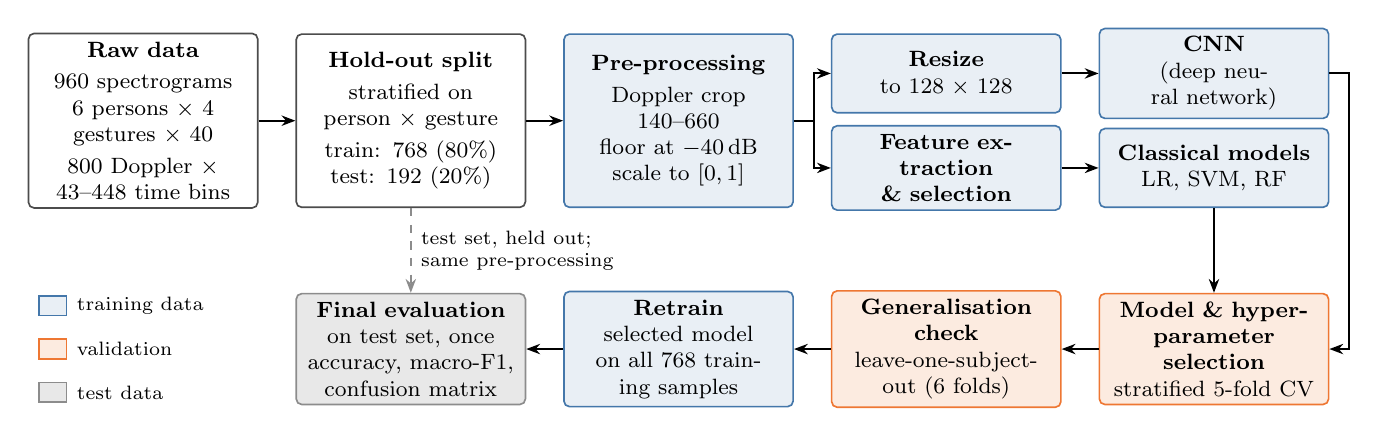
\begin{tikzpicture}[font=\footnotesize,
      box/.style={draw, rounded corners=2pt, align=center, text width=2.7cm,
        inner sep=3pt, line width=0.6pt},
      big/.style={box, minimum height=2.2cm},
      lane/.style={box, minimum height=1.0cm},
      low/.style={box, minimum height=1.4cm},
      data/.style={draw=black!70, fill=white},
      train/.style={draw=trainc, fill=trainc!12},
      val/.style={draw=valc, fill=valc!15},
      test/.style={draw=testc, fill=testc!20},
      arr/.style={-{Stealth[length=5pt]}, line width=0.7pt},
      sw/.style={draw, line width=0.6pt, minimum width=0.35cm, minimum height=0.25cm}]

    % ---- row 1: data -> split -> pre-processing -> two model branches ----
    \node[big, data]  (raw)   at (1.45, 0) {\textbf{Raw data}\\[2pt]
      960 spectrograms\\ 6 persons $\times$ 4 gestures $\times$ 40\\[2pt]
      800 Doppler $\times$ 43--448 time bins};
    \node[big, data]  (split) at (4.85, 0) {\textbf{Hold-out split}\\[2pt]
      stratified on\\ person $\times$ gesture\\[2pt]
      train: 768 (80\%)\\ test: 192 (20\%)};
    \node[big, train] (prep)  at (8.25, 0) {\textbf{Pre-processing}\\[2pt]
      Doppler crop 140--660\\ floor at $-40$\,dB\\ scale to $[0,1]$};
    \node[lane, train] (resize) at (11.65,  0.6) {\textbf{Resize}\\ to $128 \times 128$};
    \node[lane, train] (feat)   at (11.65, -0.6) {\textbf{Feature extraction\\ \& selection}};
    \node[lane, train] (cnn)    at (15.05,  0.6) {\textbf{CNN}\\ (deep neural network)};
    \node[lane, train] (clf)    at (15.05, -0.6) {\textbf{Classical models}\\ LR, SVM, RF};

    % ---- row 2 (right to left): selection -> LOSO -> retrain -> test ----
    \node[low, val]   (cv)      at (15.05, -2.9) {\textbf{Model \& hyper-\\parameter selection}\\
      stratified 5-fold CV};
    \node[low, val]   (loso)    at (11.65, -2.9) {\textbf{Generalisation check}\\
      leave-one-subject-out (6 folds)};
    \node[low, train] (retrain) at (8.25, -2.9) {\textbf{Retrain}\\
      selected model on all 768 training samples};
    \node[low, test]  (eval)    at (4.85, -2.9) {\textbf{Final evaluation}\\
      on test set, once\\ accuracy, macro-F1, confusion matrix};

    % ---- arrows ----
    \draw[arr] (raw) -- (split);
    \draw[arr] (split) -- (prep);
    \draw[arr] (prep.east) -- ++(0.25, 0) |- (resize.west);
    \draw[arr] (prep.east) -- ++(0.25, 0) |- (feat.west);
    \draw[arr] (resize) -- (cnn);
    \draw[arr] (feat) -- (clf);
    \draw[arr] (cnn.east) -- ++(0.25, 0) |- (cv.east);
    \draw[arr] (clf) -- (cv);
    \draw[arr] (cv) -- (loso);
    \draw[arr] (loso) -- (retrain);
    \draw[arr] (retrain) -- (eval);
    % test set bypasses all training and tuning
    \draw[arr, testc, dashed] (split) -- (eval)
      node[midway, right, align=left, font=\scriptsize, text=black]
      {test set, held out;\\ same pre-processing};

    % ---- legend ----
    \node[sw, train] (l1) at (0.3, -2.35) {};
    \node[anchor=west, font=\scriptsize] at (l1.east) {training data};
    \node[sw, val]   (l2) at (0.3, -2.9) {};
    \node[anchor=west, font=\scriptsize] at (l2.east) {validation};
    \node[sw, test]  (l3) at (0.3, -3.45) {};
    \node[anchor=west, font=\scriptsize] at (l3.east) {test data};
  \end{tikzpicture}
  \caption{Overview of the machine learning pipeline. The test set is
    separated before any analysis and is used only once, for the final
    evaluation. All pre-processing constants are chosen from the training
    samples only and applied to each sample separately. The CNN uses the
    resized spectrograms; the classical models use features computed on the
    spectrograms at their original length.}
  \label{fig:pipeline}
\end{figure}

% ---------- Data split: stratified hold-out test set ----------
\begin{figure}[ht]
  \centering
  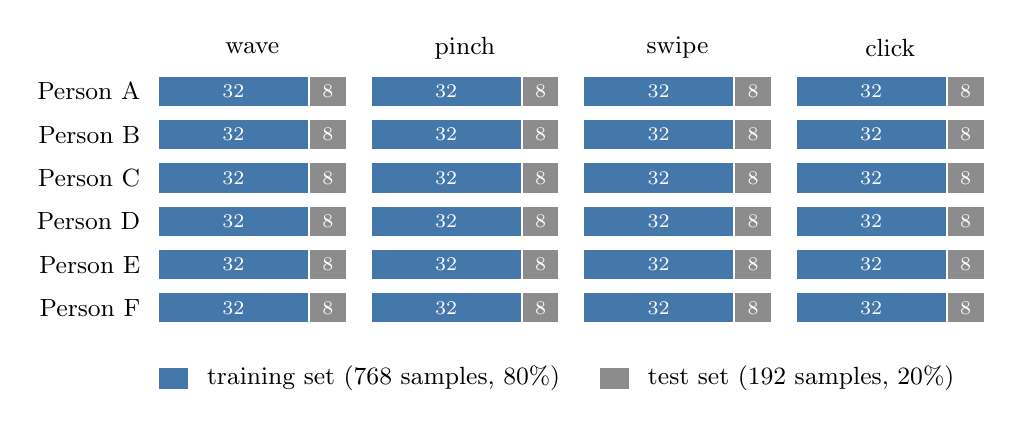
\begin{tikzpicture}[font=\small,
      seg/.style={draw=white, line width=0.8pt},
      lab/.style={font=\scriptsize, text=white}]
    % gesture column headers
    \foreach \g [count=\j from 0] in {wave, pinch, swipe, click}
      \node at ({\j*2.7+1.2}, 0.35) {\g};
    % one bar per person x gesture: 32 training (80%) + 8 test (20%)
    \foreach \p [count=\i from 0] in {A, B, C, D, E, F} {
      \node[anchor=east] at (-0.1, {-\i*0.55-0.2}) {Person \p};
      \foreach \j in {0,...,3} {
        \filldraw[seg, fill=trainc] ({\j*2.7}, {-\i*0.55}) rectangle ++(1.92, -0.4);
        \node[lab] at ({\j*2.7+0.96}, {-\i*0.55-0.2}) {32};
        \filldraw[seg, fill=testc] ({\j*2.7+1.92}, {-\i*0.55}) rectangle ++(0.48, -0.4);
        \node[lab] at ({\j*2.7+2.16}, {-\i*0.55-0.2}) {8};
      }
    }
    % legend
    \filldraw[seg, fill=trainc] (0, -3.7) rectangle ++(0.4, -0.3);
    \node[anchor=west] at (0.5, -3.85) {training set (768 samples, 80\%)};
    \filldraw[seg, fill=testc] (5.6, -3.7) rectangle ++(0.4, -0.3);
    \node[anchor=west] at (6.1, -3.85) {test set (192 samples, 20\%)};
  \end{tikzpicture}
  \caption{Stratified hold-out test set. Each of the 24 person--gesture
    combinations has 40 samples, of which 8 are assigned to the test set, so
    the test set has the same class and person balance as the full dataset.
    The test set is separated before any pre-processing and used only once,
    for the final evaluation.}
  \label{fig:split-stratified}
\end{figure}

% ---------- Data split: cross-validation folds ----------
\begin{figure}[ht]
  \centering
  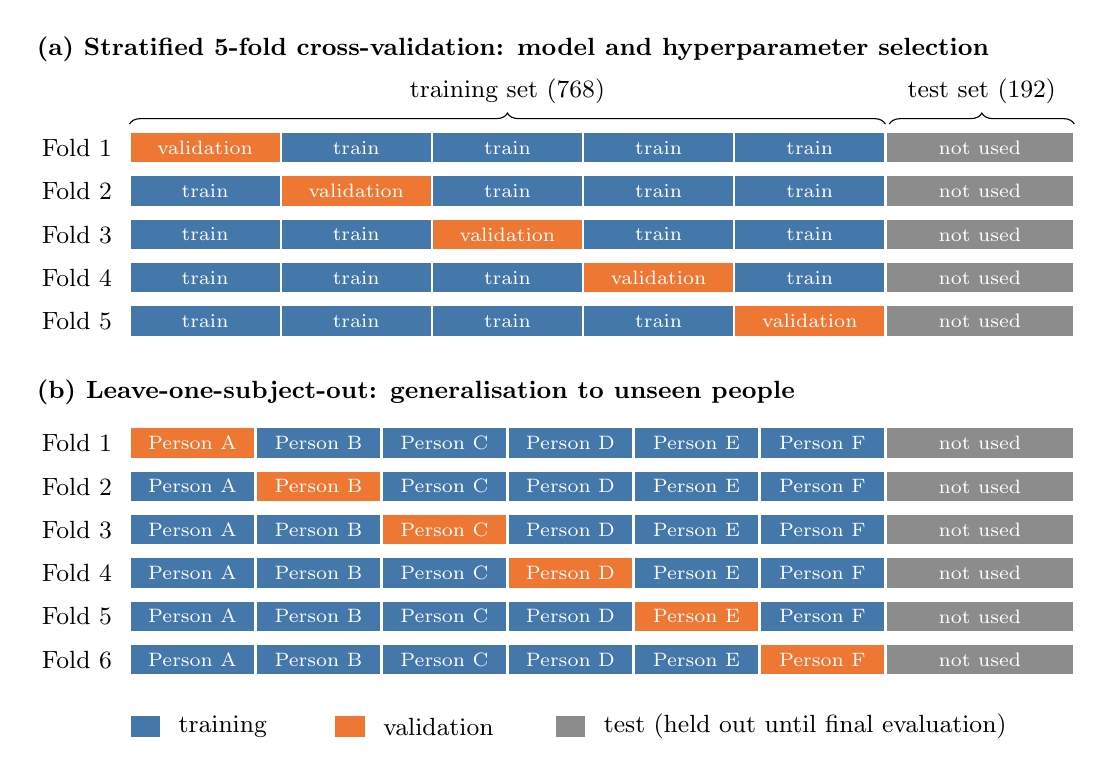
\begin{tikzpicture}[font=\small,
      seg/.style={draw=white, line width=0.8pt},
      lab/.style={font=\scriptsize, text=white}]
    % ---- (a) stratified 5-fold ----
    \node[anchor=west, font=\small\bfseries] at (-1.3, 1.05)
      {(a) Stratified 5-fold cross-validation: model and hyperparameter selection};
    \draw[decorate, decoration={brace, amplitude=4pt}] (0, 0.1) -- (9.6, 0.1)
      node[midway, above=4pt] {training set (768)};
    \draw[decorate, decoration={brace, amplitude=4pt}] (9.65, 0.1) -- (12, 0.1)
      node[midway, above=4pt] {test set (192)};
    \foreach \k in {1,...,5} {
      \pgfmathsetmacro{\y}{-(\k-1)*0.55}
      \node[anchor=east] at (-0.1, \y-0.2) {Fold \k};
      \foreach \s in {1,...,5} {
        \ifnum\s=\k \def\segcol{valc}\def\seglab{validation}%
        \else \def\segcol{trainc}\def\seglab{train}\fi
        \filldraw[seg, fill=\segcol] ({(\s-1)*1.92}, \y) rectangle ++(1.92, -0.4);
        \node[lab] at ({(\s-1)*1.92+0.96}, \y-0.2) {\seglab};
      }
      \filldraw[seg, fill=testc] (9.6, \y) rectangle ++(2.4, -0.4);
      \node[lab] at (10.8, \y-0.2) {not used};
    }
    % ---- (b) leave-one-subject-out ----
    \node[anchor=west, font=\small\bfseries] at (-1.3, -3.3)
      {(b) Leave-one-subject-out: generalisation to unseen people};
    \foreach \p [count=\k] in {A, B, C, D, E, F} {
      \pgfmathsetmacro{\y}{-3.75-(\k-1)*0.55}
      \node[anchor=east] at (-0.1, \y-0.2) {Fold \k};
      \foreach \q [count=\s] in {A, B, C, D, E, F} {
        \ifnum\s=\k \def\segcol{valc}\else \def\segcol{trainc}\fi
        \filldraw[seg, fill=\segcol] ({(\s-1)*1.6}, \y) rectangle ++(1.6, -0.4);
        \node[lab] at ({(\s-1)*1.6+0.8}, \y-0.2) {Person \q};
      }
      \filldraw[seg, fill=testc] (9.6, \y) rectangle ++(2.4, -0.4);
      \node[lab] at (10.8, \y-0.2) {not used};
    }
    % legend
    \filldraw[seg, fill=trainc] (0, -7.4) rectangle ++(0.4, -0.3);
    \node[anchor=west] at (0.5, -7.55) {training};
    \filldraw[seg, fill=valc] (2.6, -7.4) rectangle ++(0.4, -0.3);
    \node[anchor=west] at (3.1, -7.55) {validation};
    \filldraw[seg, fill=testc] (5.4, -7.4) rectangle ++(0.4, -0.3);
    \node[anchor=west] at (5.9, -7.55) {test (held out until final evaluation)};
  \end{tikzpicture}
  \caption{Validation folds on the training set (768 samples). (a)~Stratified
    5-fold cross-validation: every training sample is used for validation
    exactly once, and each fold keeps the class balance; the model and
    hyperparameters with the best mean validation score are selected.
    (b)~Leave-one-subject-out: the chosen model is trained on five people and
    validated on the sixth, which measures generalisation to people not seen
    during training. In both schemes the test set is never used.}
  \label{fig:split-folds}
\end{figure}

% =====================================================================
\section{Task 1: Data Pre-processing and Feature Extraction}
\label{sec:task1}
% =====================================================================
\placeholder{%
\textbf{Required content:} selected options for pre-processing and possible
feature extraction, \emph{argumentation for the selection}, and
\emph{results}. \textbf{Rubric: Data analysis \& pre-processing (10\%) +
Feature selection (15\%).} Explain the implementation without showing complete
code; short key code steps are acceptable.}

\subsection{Exploratory Data Analysis}
\placeholder{%
\begin{itemize}
  \item Example spectrogram per class (magnitude in dB) -- one figure with 4
        subplots, labelled axes (Doppler/velocity bin, time), colourbar.
  \item Statistics: number of samples per class and per person, distribution
        of spectrogram lengths, dynamic range of dB values, outliers / corrupt
        or empty samples (NaN, inf, all-zero), inter-subject variability.
  \item Observations that motivate the pre-processing choices below.
\end{itemize}}

\begin{figure}[h]
  \centering
  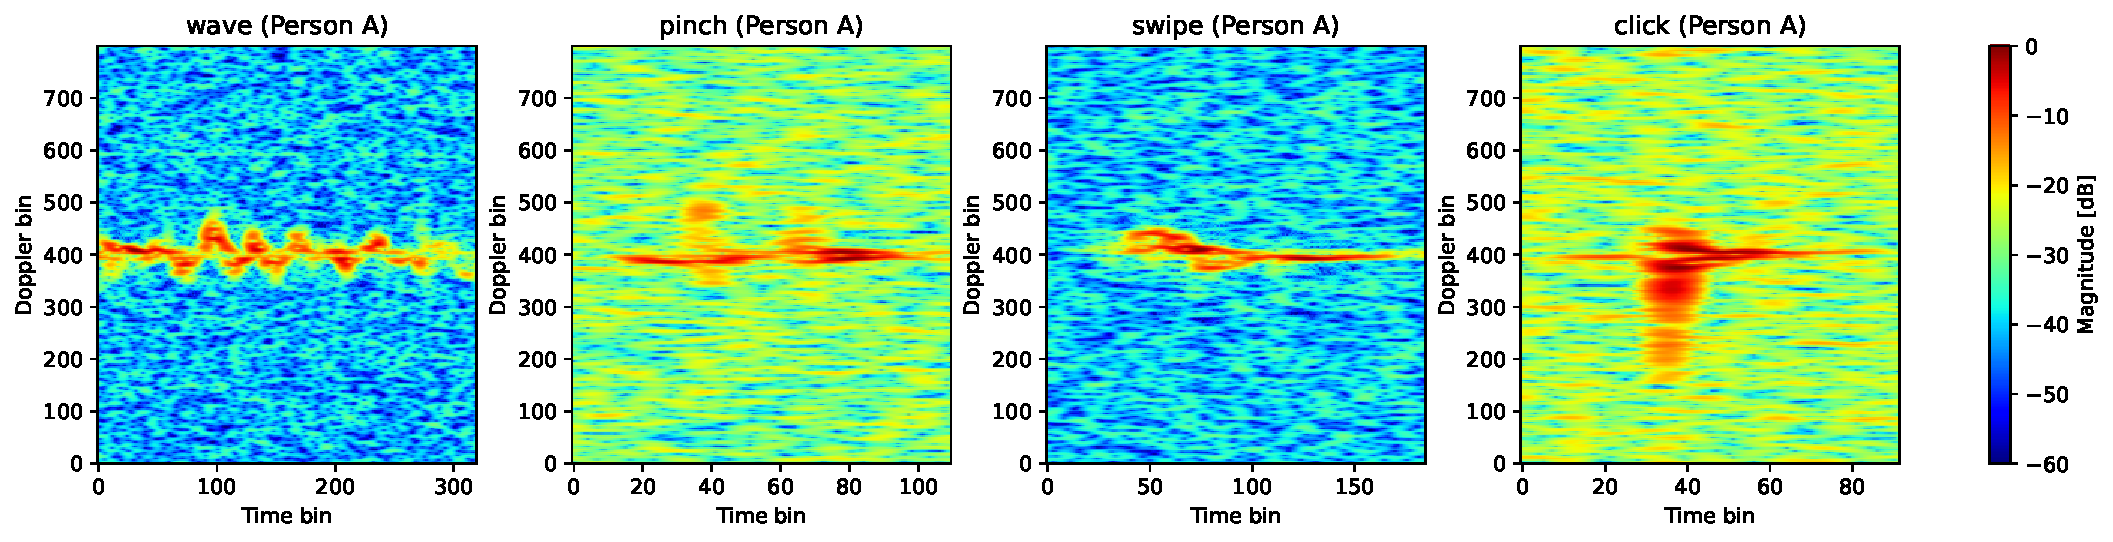
\includegraphics[width=\linewidth]{figures/spectrograms.pdf}
  \caption{Example micro-Doppler spectrogram for each gesture (magnitude in dB).}
  \label{fig:spectrograms}
\end{figure}

\begin{figure}[h]
  \centering
  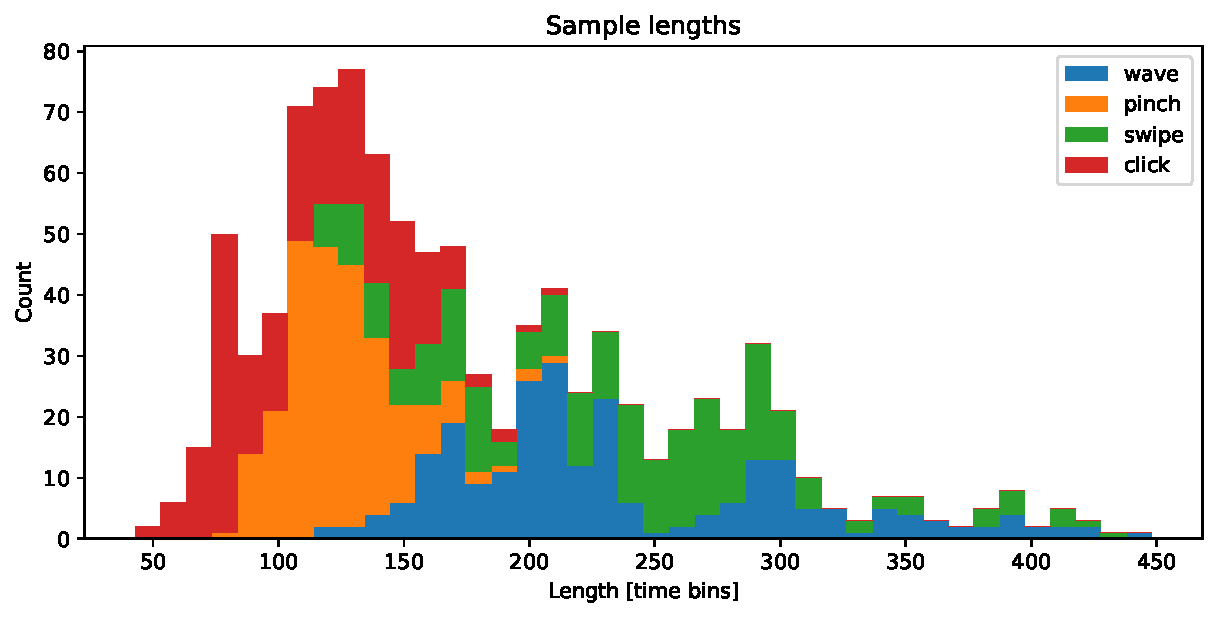
\includegraphics[width=0.7\linewidth]{figures/length_histogram.pdf}
  \caption{Distribution of sample lengths (number of time bins), stacked per gesture.}
  \label{fig:length_histogram}
\end{figure}

\begin{figure}[h]
  \centering
  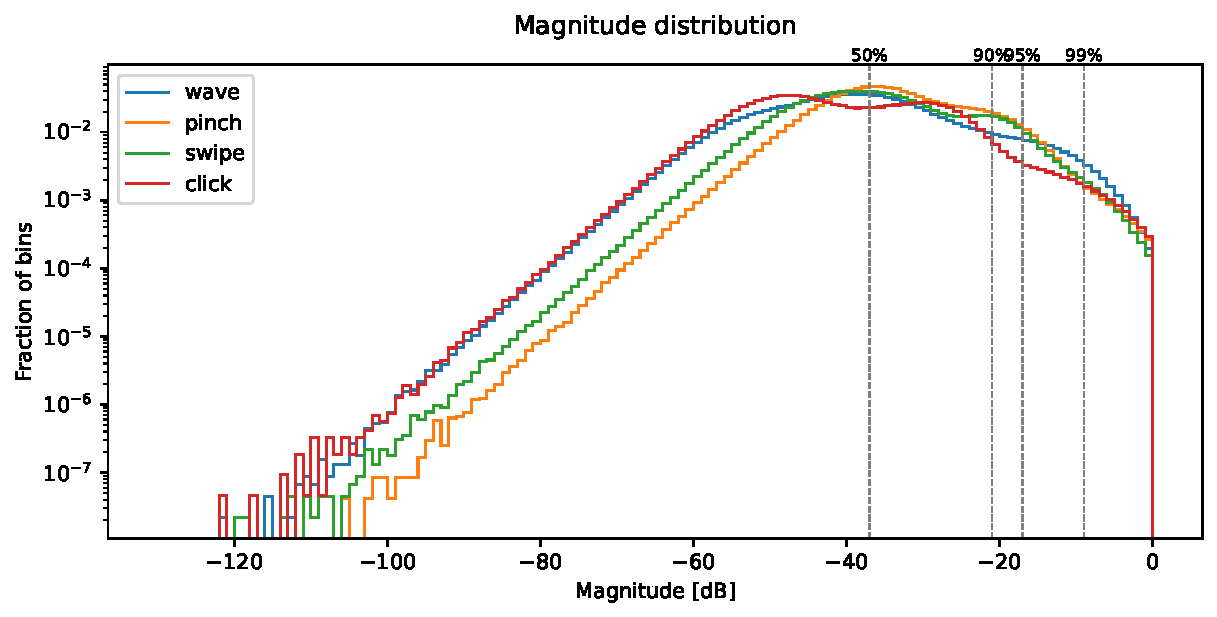
\includegraphics[width=0.7\linewidth]{figures/magnitude_histogram.pdf}
  \caption{Distribution of magnitude values over all time-Doppler bins, per gesture (log scale).}
  \label{fig:magnitude_histogram}
\end{figure}

\subsection{Pre-processing}
\placeholder{%
Describe and \emph{justify} each step chosen (the assignment lists data
cleaning, normalisation, standardisation of spectrograms treated as images).
Examples to consider:
\begin{itemize}
  \item Data cleaning: handling NaN/inf, removing corrupted samples.
  \item Handling variable time length: cropping, zero/min-padding, resizing /
        interpolation to a fixed size.
  \item Dynamic-range clipping (e.g.\ floor at max$-X$\,dB) to suppress noise.
  \item Normalisation / standardisation (per-sample min--max, global z-score
        fitted on training data only -- avoid leakage).
  \item Optional: Doppler cropping around zero velocity, denoising, data
        augmentation for the DNN (time shift, noise) -- training set only.
\end{itemize}
Report the effect of each choice (figure before/after, and/or ablation
showing impact on validation accuracy).}

\subsection{Feature Extraction and Selection}
\placeholder{%
Optional in the assignment but worth \textbf{15\%} of the rubric -- argue why
you do/do not use explicit features (e.g.\ DNN on raw images vs.\ handcrafted
features for classical models). Inspiration suggested by the lecturer:
\begin{enumerate}
  \item \textbf{Envelope features} -- Amin, Zeng \& Shan, \emph{Hand Gesture
        Recognition based on Radar Micro-Doppler Signature Envelopes}, IEEE
        RadarConf 2019 \cite{amin2019}: upper/lower/central envelopes of the
        spectrogram.
  \item \textbf{Centroid and bandwidth} -- Fioranelli, Ritchie \& Griffiths,
        IET RSN 2016 \cite{fioranelli2016}, Sec.~3.2: Doppler centroid and
        bandwidth over time and their statistical moments (note: originally for
        a different task).
  \item \textbf{Chebyshev moments} -- Pallotta et al., IEEE MetroAeroSpace 2021
        \cite{pallotta2021}.
\end{enumerate}
Other options: statistical features (mean, variance, skewness, kurtosis,
energy, entropy), PCA, image-texture features. Explain:
\begin{itemize}
  \item Feature definitions (equations where useful).
  \item Feature selection / dimensionality reduction method (e.g.\ correlation
        analysis, mutual information, recursive feature elimination, PCA
        explained variance) and why.
  \item Results: feature distributions per class, separability plots
        (e.g.\ pair plots, t-SNE/PCA scatter), feature importance ranking.
\end{itemize}}

\begin{table}[h]
  \centering
  \caption{Extracted features (example layout).}
  \label{tab:features}
  \begin{tabular}{@{}llc@{}}
    \toprule
    Feature group & Description & \# features \\
    \midrule
    Envelope        & \ldots & -- \\
    Centroid/bandwidth & \ldots & -- \\
    Chebyshev moments  & \ldots & -- \\
    \bottomrule
  \end{tabular}
\end{table}

\subsection{Task 1 Results}
\placeholder{%
Summarise the outcome of Task~1: final input representation(s) fed to each
model, final feature set and its size, key plots showing class separability,
and a short discussion of what worked and what did not.}

% =====================================================================
\section{Task 2: Model Development, Validation and Comparison}
\label{sec:task2}
% =====================================================================
\placeholder{%
\textbf{Required content:} argumentation for the model(s) developed,
validations, results, comparisons. \textbf{Rubric: Model selection (20\%) +
Hyperparameter tuning (20\%) + Performance indicators (10\%) + Appropriate use
of data (10\%).} \textbf{At least one model MUST be a deep neural network --
otherwise the report is inadmissible (FAIL).} Explain implementation and reason
about results; no full code.}

\subsection{Model Selection and Design}
\placeholder{%
\begin{itemize}
  \item Candidate models and \emph{why} each was chosen. Suggested mix: a
        simple baseline (e.g.\ logistic regression / $k$-NN), classical
        models on handcrafted features (e.g.\ SVM, random forest), and the
        mandatory DNN (e.g.\ CNN on spectrogram images, or MLP on features).
  \item DNN architecture: layers, filter sizes, activations, pooling,
        dropout/batch-norm, number of parameters; architecture figure or table.
  \item Design arguments linked to the data (small dataset $\rightarrow$
        overfitting risk, regularisation, model capacity).
\end{itemize}}

\subsection{Validation Procedure and Performance Indicators}
\placeholder{%
\begin{itemize}
  \item Validation strategy and justification: e.g.\ stratified $k$-fold CV,
        hold-out validation, leave-one-subject-out CV (generalisation to unseen
        persons). Explain how the test set stays unseen until the end.
  \item Loss function(s) (e.g.\ cross-entropy), optimiser, learning rate,
        batch size, epochs, \textbf{convergence/stopping criteria} (early
        stopping on validation loss).
  \item Metrics and why: accuracy, per-class precision/recall, macro-F1,
        confusion matrix; mean $\pm$ std over folds.
  \item Training/validation loss and accuracy curves for the DNN to show
        convergence and detect over-/under-fitting.
\end{itemize}}

\subsection{Hyperparameter Tuning}
\placeholder{%
Worth \textbf{20\%}. For each model list tuned hyperparameters, search space,
search method (grid / random / Bayesian search, e.g.\
\texttt{GridSearchCV}), the CV used inside the search, and the selected values.
Show validation performance vs.\ key hyperparameters (plot or table) and
comment on sensitivity.}

\begin{table}[h]
  \centering
  \caption{Hyperparameter search space and selected values (example layout).}
  \label{tab:hyper}
  \begin{tabular}{@{}llll@{}}
    \toprule
    Model & Hyperparameter & Search space & Selected \\
    \midrule
    SVM & $C$, kernel, $\gamma$ & \ldots & \ldots \\
    Random forest & \# trees, max depth & \ldots & \ldots \\
    CNN & learning rate, dropout, \# filters & \ldots & \ldots \\
    \bottomrule
  \end{tabular}
\end{table}

\subsection{Results and Comparison}
\placeholder{%
\begin{itemize}
  \item Table comparing all models: validation (mean $\pm$ std) and final test
        performance; optionally training time / number of parameters.
  \item Confusion matrix of the best model on the test set; discuss which
        gestures get confused and why (physical motion similarity).
  \item Optional: per-person performance to discuss inter-subject
        generalisation.
  \item Argue the choice of the \textbf{final model}, trade-offs (accuracy vs.\
        complexity, handcrafted features vs.\ end-to-end DNN).
\end{itemize}}

\begin{table}[h]
  \centering
  \caption{Model comparison (example layout).}
  \label{tab:results}
  \begin{tabular}{@{}lccc@{}}
    \toprule
    Model & Val.\ accuracy (mean $\pm$ std) & Test accuracy & Test macro-F1 \\
    \midrule
    Baseline        & -- & -- & -- \\
    SVM (features)  & -- & -- & -- \\
    Random forest   & -- & -- & -- \\
    CNN (spectrogram) & -- & -- & -- \\
    \bottomrule
  \end{tabular}
\end{table}

\begin{figure}[h]
  \centering
  \fbox{\parbox[c][3.5cm][c]{0.45\linewidth}{\centering Confusion matrix (test)}}
  \hfill
  \fbox{\parbox[c][3.5cm][c]{0.45\linewidth}{\centering DNN train/val curves}}
  \caption{(Left) Confusion matrix of the final model on the test set.
    (Right) Training and validation loss/accuracy of the DNN.}
  \label{fig:results}
\end{figure}

% =====================================================================
\section{Conclusions}
\label{sec:conclusions}
% =====================================================================
\placeholder{%
\textbf{Hard limit: less than 200 words.} Answer the problem statement:
best model and its test performance, the most influential pre-processing /
feature choices, limitations (small dataset, subject variability, test-set
size), and possible future work (e.g.\ complex-valued input, data augmentation,
transfer learning).}

% =====================================================================
% References (on a separate page, not counted towards 10-page limit)
% =====================================================================
\clearpage
\pagenumbering{roman} % distinguish from the counted body pages
\begin{thebibliography}{9}
\bibitem{dopnet}
  UCL Radar Group, ``DopNet radar hand-gesture dataset,''
  \url{https://github.com/UCLRadarGroup/DopNet}.
\bibitem{amin2019}
  M.~G. Amin, Z.~Zeng, and T.~Shan, ``Hand gesture recognition based on radar
  micro-Doppler signature envelopes,'' in \emph{Proc.\ IEEE Radar Conf.},
  2019, pp.~1--6.
\bibitem{fioranelli2016}
  F.~Fioranelli, M.~Ritchie, and H.~Griffiths, ``Centroid features for
  classification of armed/unarmed multiple personnel using multistatic human
  micro-Doppler,'' \emph{IET Radar, Sonar \& Navigation}, vol.~10,
  pp.~1702--1710, 2016.
\bibitem{pallotta2021}
  L.~Pallotta, M.~Cauli, C.~Clemente, F.~Fioranelli, G.~Giunta, and A.~Farina,
  ``Classification of micro-Doppler radar hand-gesture signatures by means of
  Chebyshev moments,'' in \emph{Proc.\ IEEE MetroAeroSpace}, 2021,
  pp.~182--187.
\end{thebibliography}

\end{document}
